\documentclass{article}
\usepackage[utf8]{inputenc}
\usepackage{amsmath}
\usepackage{graphicx}
\graphicspath{ {./images/} }

\title{Tarea 04 de Circuitos Lineales I}
\author{Gabriel Gamboa Vargas}
\date{Noviembre 2021}

\begin{document}
\maketitle
\section{Ejercicio 1 y 4}
Se utiliza el programa Micro Cap. Se juntan ambos ejercicios para tener más claridad.\\
Se referirá a las corrientes de rama por el nombre del elemento de circuito por el cual la corriente circula. Se muestra el circuito por partes.\\
 Los valores en forma tabulada son:\\ \\    
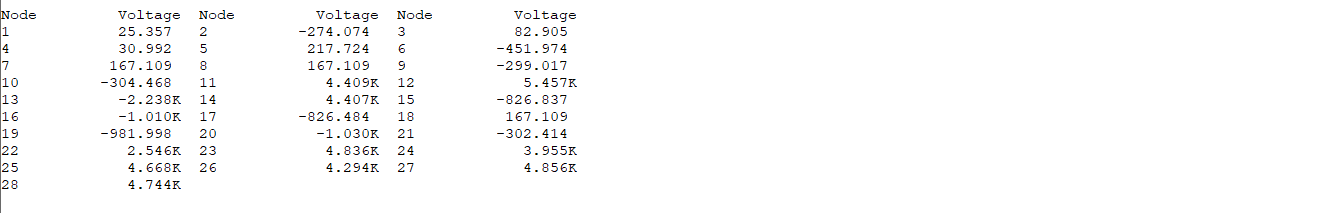
\includegraphics[]{images/tensionesMicroCap.PNG}\\ 
A continuación se muestra donde están ubicados estos valores y se utilizan para calcular las corrientes de rama.\\
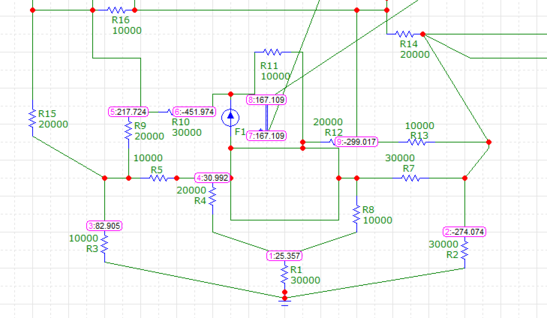
\includegraphics[]{images/MicroCap1_75.PNG}\\ 
El nombre del nodo está escrito en la izquierda y su tensión de nodo luego de los dos puntos.\\ \\
$I(F1) =  70.62m A$\\
$I(R1) = v1/R1 = 845u A$\\
$I(R2) = v2/R3 = -247.074 A$\\
$I(R3) = v3/R1 = 8.291m A$\\
$I(R4) = \frac{v4-v1}{R2} = -281.748u A$\\
$I(R5) = \frac{v3-v4}{R1} = 5.191m A$\\
$I(R7) = \frac{v4-v2}{R3} = 10.169m A$\\
$I(R8) = \frac{v4-v2}{R1} = 563.496u A$\\
$I(R9) = \frac{v5-v3}{R2} = 6.741m A$\\
$I(R10) = \frac{v5-v6}{R3} = 22.323m A$\\
$I(R11) = \frac{v4-v6}{R1} = 48.297m A$\\
$I(R12) = \frac{v4-v9}{R2} = 16.5m A$\\
$I(R13) = \frac{v2-v9}{R1} = 2.494m A$\\
$I(R14) = \frac{v2-v9}{R2} = 1.247m A$\\
$I(R15) = \frac{v5-v3}{R2} = 6.741m A$\\
$I(R16) = \frac{v5-v9}{R1} = 51.674m A$\\ \\
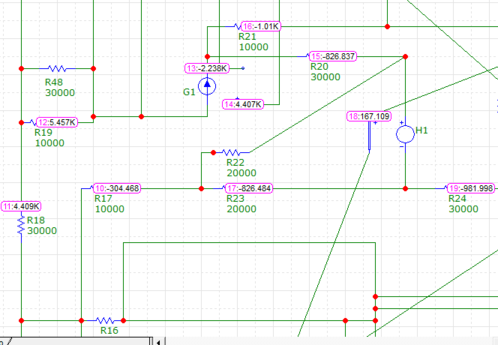
\includegraphics[]{images/MicroCap2_75.PNG}\\ \\
$I(G1) = 169.836m A$\\
$I(H1) = 20.917m A$\\
$I(R17) = \frac{v5-v19}{R1} = 52.219m A$\\ 
$I(R18) = \frac{v5-v11}{R3} = 139.699m A$\\ 
$I(R19) = \frac{v12-v11}{R1} = 104.838m A$\\ 
$I(R48) = \frac{v12-v11}{R3} = 34.946m A$\\ 
$I(R22) = \frac{v10-v15}{R2} = 26.118m A$\\ 
$I(R23) = \frac{v10-v17}{R2} = 26.101m A$\\ 
$I(R21) = \frac{v16-v13}{R1} = 122.801m A$\\ 
$I(R20) = \frac{v15-v13}{R3} = 47.035m A$\\ 
$I(R24) = \frac{v17-v19}{R3} = 51.674m A$\\ 
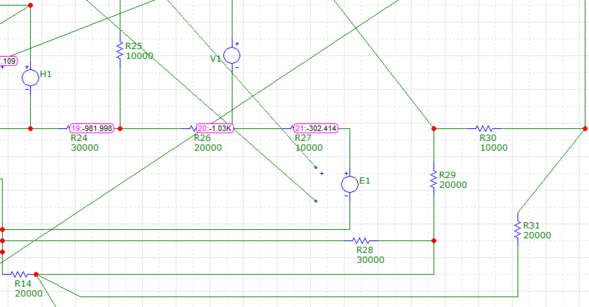
\includegraphics[]{images/MicroCap3_75.PNG}\\ \\
$I(E1) = 72.748m A$\\
$I(v1) = 75.142m A$\\
$I(R25) = \frac{v19-v16}{R1} = 2.789m A$\\ 
$I(R26) = \frac{v19-v20}{R2} = 2.395m A$\\ 
$I(R27) = \frac{v21-v20}{R1} = 72.748m A$\\ 
$I(R28) = \frac{v2-v9}{R3} = 831.45u A$\\ 
$I(R29) = \frac{v2-v16}{R2} = 36.791m A$\\ 
$I(R30) = \frac{v8-v16}{R1} = 117.7m A$\\ 
$I(R31) = \frac{v8-v2}{R2} = 22.059m A$\\ 
$I(R32) = \frac{v8-v16}{R3} = 39.233m A$\\ 
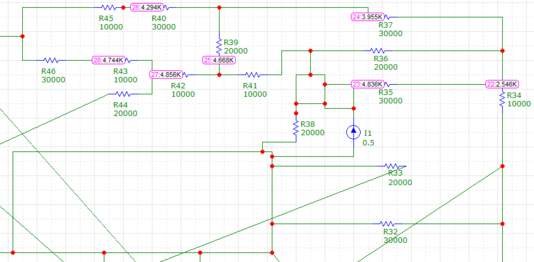
\includegraphics[]{images/MicroCap4_75.PNG}\\ \\
$I(R33) = \frac{v18-v16}{R2} = 58.85m A$\\ 
$I(R34) = \frac{v22-v8}{R1} = 237.842m A$\\ 
$I(R35) = \frac{v23-v22}{R3} = 76.35m A$\\ 
$I(R36) = \frac{v23-v22}{R2} = 114.525m A$\\ 
$I(R37) = \frac{v24-v22}{R3} = 46.968m A$\\ 
$I(R38) = \frac{v23-v16}{R2} = 39.233m A$\\ 
$I(R39) = \frac{v25-v24}{R2} = 35.658m A$\\ 
$I(R40) = \frac{v26-v24}{R3} = 11.31m A$\\ 
$I(R41) = \frac{v23-v25}{R1} = 16.83m A$\\ 
$I(R42) = \frac{v27-v25}{R1} = 18.828m A$\\ 
$I(R43) = \frac{v27-v28}{R1} = 11.225m A$\\ 
$I(R44) = \frac{v12-v27}{R2} = 30.053m A$\\ 
$I(R45) = \frac{v14-v26}{R1} = 11.31m A$\\ 
$I(R46) = \frac{v28-v14}{R3} = 11.225m A$\\ 
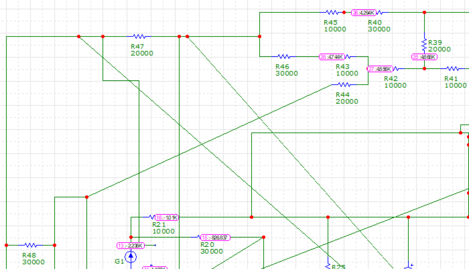
\includegraphics[]{images/MicroCap5_67.PNG}\\ \\
$I(R47) = \frac{v11-v14}{R2} = 84.918u A$\\ 
\section{Ejercicio 2 y 4}
Se utiliza el programa Ltspice, note que las tensiones de nodos están nombradas de la misma forma que en el circuito diseñado en Micro Cap, los resistores no tienen la misma numeración. Se mostrarán los datos tabulados y luego las imágenes del circuito.\\ \\
Los valores de las tensiones de nodo son:\\ 
\includegraphics[]{images/ltspicetensiones.PNG}\\ \\
Los valores de las corrientes de rama son: \\ \\
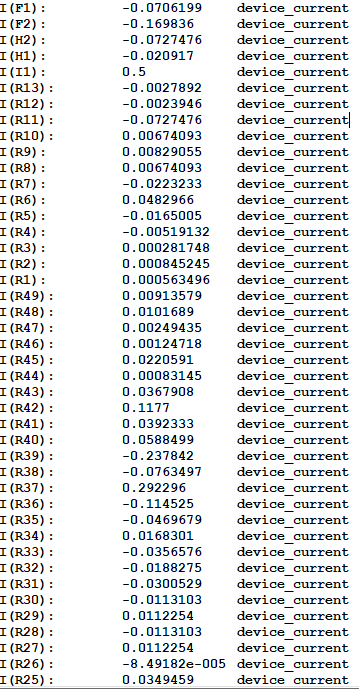
\includegraphics[]{images/ramas1.PNG}\\ \\
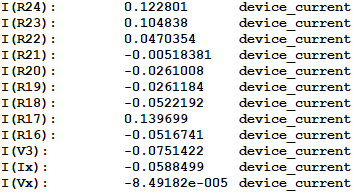
\includegraphics[]{images/ramas2.PNG}\\ \\
Puede encontrar donde se encuentran estos valores en las siguientes capturas.\\
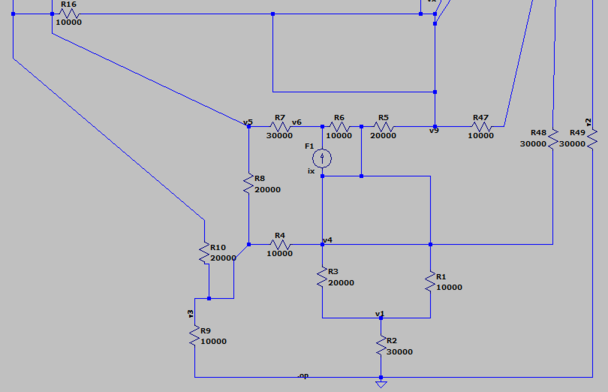
\includegraphics[]{images/ltspice1_75.PNG}\\ \\
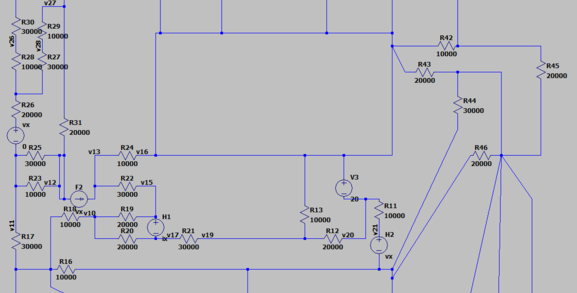
\includegraphics[]{images/ltspice2_75.PNG}\\ \\
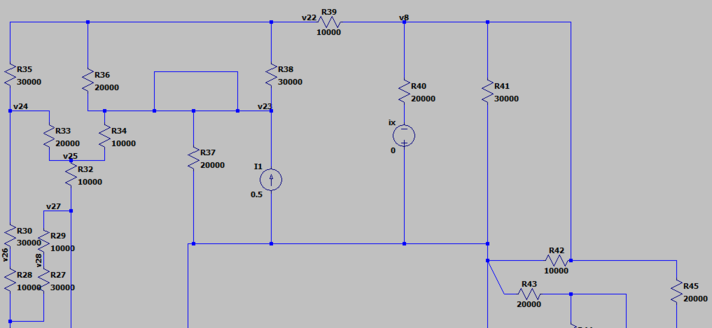
\includegraphics[]{images/ltspice3_70.PNG}\\ \\
\section{Ejercicio 3}
Se utiliza el siguiente archivo SPICE, creado del código SPICE del circuito de Micro Cap.\\
Ejercicio 3\\
E1 21 9 14 11 2\\
F1 4 6 VF1 1.2\\
G1 12 13 14 11 0.1\\
H1 15 17 VH1 {6}\\
I1 16 23 DC 0.5\\
R1 0 1 30000\\
R2 2 0 30000\\
R3 3 0 10000\\
R4 4 1 20000\\
R5 3 4 10000\\
R7 4 2 30000\\
R8 1 4 10000\\
R9 3 5 20000\\
R10 6 5 30000\\
R11 4 6 10000\\
R12 4 9 20000\\
R13 2 9 10000\\
R14 2 9 20000\\
R15 3 5 20000\\
R16 9 5 10000\\
R17 10 5 10000\\
R18 5 11 30000\\
R19 12 11 10000\\
R20 15 13 30000\\
R21 16 13 10000\\
R22 15 10 20000\\
R23 17 10 20000\\
R24 19 17 30000\\
R25 19 16 10000\\
R26 20 19 20000\\
R27 21 20 10000\\
R28 2 9 30000\\
R29 2 16 20000\\
R30 8 16 10000\\
R31 2 8 20000\\
R32 8 16 30000\\
R33 18 16 20000\\
R34 8 22 10000\\
R35 22 23 30000\\
R36 22 23 20000\\
R37 22 24 30000\\
R38 16 23 20000\\
R39 25 24 20000\\
R40 24 26 30000\\
R41 23 25 10000\\
R42 25 27 10000\\
R43 27 28 10000\\
R44 27 12 20000\\
R45 26 14 10000\\
R46 28 14 30000\\
R47 14 11 20000\\
R48 12 11 30000\\
RE1 14 11 1G;added by E1\\
RG1 14 11 1G ;added by G1\\
V1 16 20 DC 20\\
VF1 7 8 0 ;added by F1\\
VH1 18 7 0 ;added by H1\\
*\\

*\\
*\\
.DC 0 0 0 0\\
*\\
.PROBE\\
.END\\

Se utiliza el comando "source two.cir" para cargar el circuito, una vez cargado exitosamente se usa el comando "op" para simular corriente continua. Después se usa el comando "print all" para mostrar todas las tensiones de nodo, note que está enumerado de la misma forma que el circuito de Ltspice y el de Micro Cap.\\
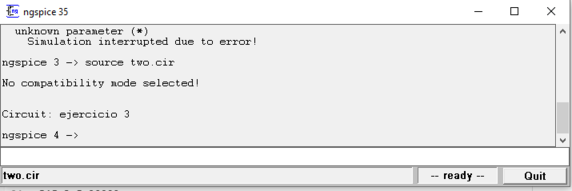
\includegraphics[]{images/ngspice1_70.PNG}\\ \\
$e+x$ representa un factor de $10^x$ \\  
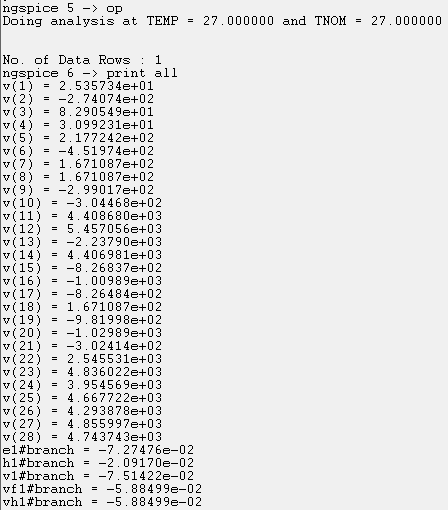
\includegraphics[]{images/ngspice2.PNG}\\ \\
El código fuente SPICE de Ltspice es:\\ \\ 
R16 v9 v5 10000\\
R17 v11 v5 30000\\
R18 v10 v5 10000\\
R19 v15 v10 20000\\
R20 v17 v10 20000\\
H1 v15 v17 ix 6\\
R21 v19 v17 30000\\
R22 v15 v13 30000\\
R23 v12 v11 10000\\
F2 v12 v13 vx 2000\\
R24 v16 v13 10000\\
R25 v12 v11 30000\\
vx N003 v11 0\\
R26 N002 N003 20000\\
R27 v28 N002 30000\\
R28 v26 N002 10000\\
R29 v27 v28 10000\\
R30 v24 v26 30000\\
R31 v27 v12 20000\\
R32 v25 v27 10000\\
R33 v24 v25 20000\\
R34 v23 v25 10000\\
R35 v22 v24 30000\\
R36 v22 v23 20000\\
R37 v23 v16 20000\\
R38 v22 v23 30000\\
I1 v16 v23 0.5\\
R39 v8 v22 10000\\
R40 v8 N001 20000\\
V§ix v16 N001 0\\
R41 v8 v16 30000\\
R42 v8 v16 10000\\
R43 v2 v16 20000\\
R44 v2 v9 30000\\
R45 v8 v2 20000\\
R46 v2 v9 20000\\
R47 v2 v9 10000\\
R48 v4 v2 30000\\
R49 0 v2 30000\\
R1 v4 v1 10000\\
R2 v1 0 30000\\
R3 v4 v1 20000\\
R4 v4 v3 10000\\
R5 v9 v4 20000\\
F1 v4 v6 ix 1.2\\
R6 v4 v6 10000\\
R7 v6 v5 30000\\
R8 v5 v3 20000\\
R9 v3 0 10000\\
R10 v5 v3 20000\\
H2 v21 v9 vx 40000\\
R11 v20 v21 10000\\
V3 v16 v20 20\\
R12 v20 v19 20000\\
R13 v16 v19 10000\\
.op\\
.backanno\\
.end\\


\end{document}